%!TEX program = xelatex
%%%%%%%%%%%%%%%%%%%%%%%这是导言部分的开始%%%%%%%%

%========= 导言部分声明文档的类型=================
\documentclass{article}

	%=========导言部分可可以加载宏包=================
	\usepackage{amsmath}                % 数学公式排版宏包
	\usepackage{amssymb}                % 数学符号命令宏包
	\usepackage{amsthm}                 % 数学定理宏包
	\usepackage[UTF8]{ctex}             % 中文输入宏包
	\usepackage[a4paper]{geometry}      % 页面设置宏包
	\usepackage{setspace}               % 行间距宏包
	\usepackage{graphicx}               % 图片宏包
	\usepackage{listings}               % 代码宏包
	\usepackage{color}					% 颜色宏包
	\usepackage{xcolor}                 % 颜色处理宏包
	\usepackage{float}                  % 浮动对象式样宏包
	\usepackage{fontspec}
	
	%=========页面设置==============================
	\geometry{left=1cm,right=1cm,top=1cm,bottom=2cm}
	\onehalfspacing
	\setlength\parindent{0em}
	
	%=========代码格式设置============================
	\definecolor{dkgreen}{rgb}{0,0.6,0}
	\definecolor{gray}{rgb}{0.5,0.5,0.5}
	\definecolor{mauve}{rgb}{0.58,0,0.82}
	% \setmonofont{Consolas}
	\lstset{
		numbers = left, 	
		numberstyle = \color{gray}, 
		keywordstyle = \color{blue},
		commentstyle = \color{dkgreen}, 
		stringstyle = \color{mauve},
		basicstyle = \ttfamily,
		breaklines = true,
		frame = shadowbox, % 阴影效果
		rulesepcolor = \color{ red!20!green!20!blue!20} ,
		escapeinside = ``, % 英文分号中可写入中文
		xleftmargin = 2em,xrightmargin=2em, aboveskip=1em,
		framexleftmargin = 2em
	} 

%=========导言部分可以定义标题信息===============
\title{组会报告}
\author{徐益}
\date{\today}

%%%%%%%%%%%%%%%%%%%%%%%这是导言部分的结束%%%%%%%%%

%%%%%%%%%%%%%%%%%%%%%%%这是正文部分的开始%%%%%%%%%
\begin{document}
	
%=========生成标题================================
\maketitle

%=========开始正文的输入==========================

%===========第一节=================
\section{本周工作内容}

1. 配置服务器10.129.4.107/10.129.4.108

2. 实现DPDK裸数据传输

3. 实现数据处理+DPDK本地调试

%===========第一节=================
\section{数据处理+DPDK本地调试模型}
\begin{figure}[H]
	\centering
	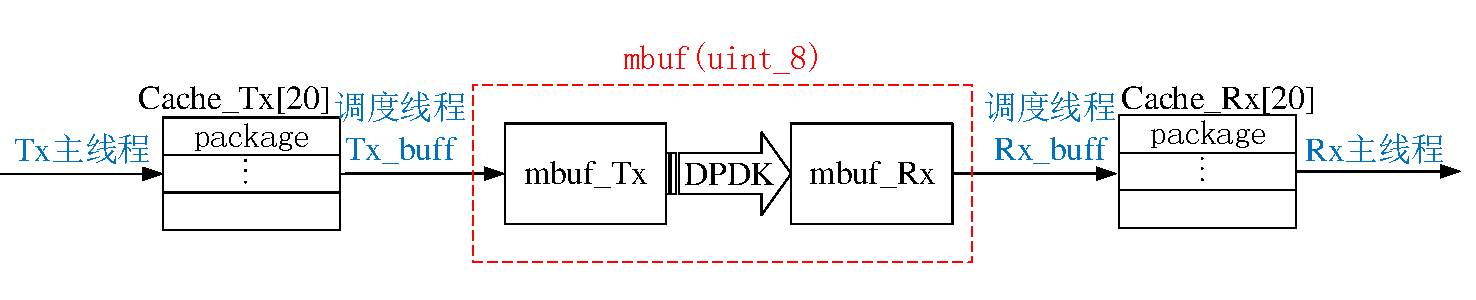
\includegraphics[width = \textwidth]{frame_mbuf.pdf}
	\caption{数据处理+DPDK本地调试模型}
\end{figure}
\begin{figure}[H]
	\centering
	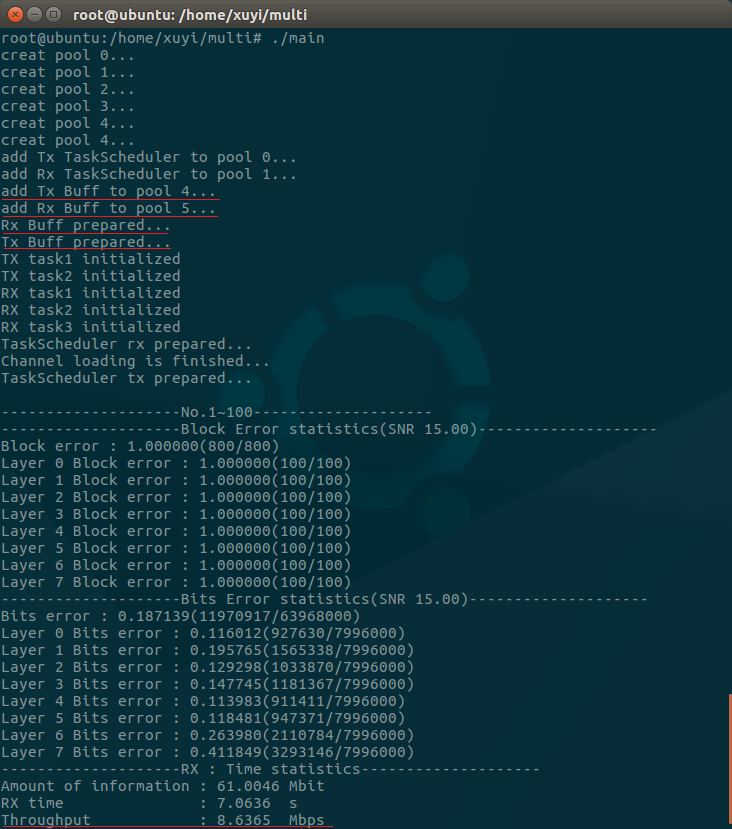
\includegraphics[width = .45\textwidth]{multi_result.png}
	\caption{服务器运行结果}
\end{figure}

%===========第二节=================
\section{调试DPDK裸数据传输时的问题(已解决)}
1. 异地生成的可执行文件无法获得部分权限。\\
方案:在服务器上编译代码。\\

2. 服务器缺少部分编译组件。\\
方案:使用代理服务器:export http\_proxy=http://121.248.50.249:808\\

3. 服务器端调试代码困难。\\
方案:使用本地调试模型。\\

%===========第三节=================
\section{调试数据处理+DPDK本地模型时的问题(已解决)}
1. 数据处理系统整体改写后,debug困难。\\
方案:分步将新增线程融入源系统,保证每一步改写都可执行验证。\\

2. 重复定义问题。\\
方案:将config.h中常量由const类型改为宏(\#define)\\

3. 系统默认栈空间不足,无法模拟mbuf。\\
方案:使用堆空间(malloc)。\\

4. 调度线程无法进入主循环中的处理区域。\\
方案:在条件处理区域前加入等待信号量函数(sem\_wait),第一次满足条件后唤醒。\\

5. 读取约束和写入约束混乱。\\
方案:将Cache中package数作为读约束,将系统中所有存在的package数作为写约束。\\

%===========第四节=================
\section{其他改进方向}
1. 处理内存泄露问题。\\

2. 引入进程结束信号。\\

3. 加入时延分析模块。\\

%===========存在问题=================
\section{仍存在问题}
1. 结构体内指针所指的堆内容无法在不同文件访问。\\
暂时方案:各个线程写在同一个文件中。\\

2. 实验室PC无法添加超过4个线程。\\
暂时方案:使用笔记本调试代码。\\
\begin{figure}[H]
	\centering
	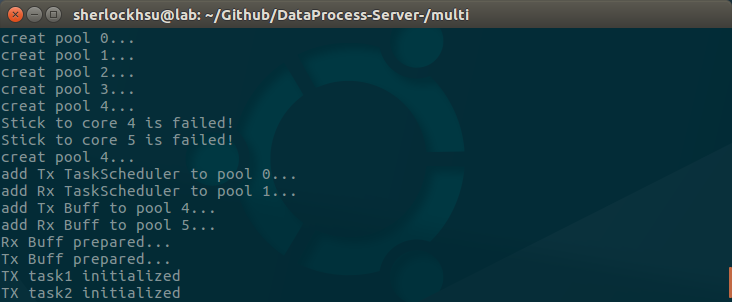
\includegraphics[width = .8\textwidth]{fail_result.png}
	\caption{本地运行结果}
\end{figure}

%===========下周计划=================
\section{下周计划}
1. 继续完成数据处理+DPDK系统

2. 学习LDPC相关内容

\end{document}
%%%%%%%%%%%%%%%%%%%%%%%这是正文部分的结束%%%%%%%%%%%%